\documentclass[a4paper, 12pt]{report}
\usepackage{cmap}
\usepackage[T2A]{fontenc}
\usepackage[utf8]{inputenc}
\usepackage[english,russian]{babel}
\usepackage{listings}
\usepackage{amsmath}
\usepackage{float}
\usepackage{csquotes}
\usepackage{graphicx}
\graphicspath{ {./images/} }
\usepackage{xcolor}
\definecolor{buzzlightyear}{HTML}{8757A5}
\definecolor{grass}{HTML}{738D06}
\definecolor{literal}{HTML}{F18A2B}
\definecolor{commentcolor}{HTML}{8E908B}

\lstdefinestyle{habrstyle}{
	backgroundcolor=\color{white},
	commentstyle=\color{commentcolor},
	keywordstyle=\bfseries\color{buzzlightyear},
	numberstyle=\tiny\color{commentcolor},
	stringstyle=\color{grass},
	basicstyle=\ttfamily\footnotesize,
	breakatwhitespace=false,         
    	breaklines=true,                 
   	captionpos=b,                    
    	keepspaces=true,                 
    	numbers=left,                    
    	numbersep=7pt,                  
    	showspaces=false,                
    	showstringspaces=false,
   	showtabs=false,                  
    	tabsize=3
}

\lstset{style=habrstyle}

\author{3530901/80201, Шелаев Н. Р.}
\title{Лабораторная работа № 7. Дискретное преобразование Фурье.}
\date{\today}

\begin{document}
	\maketitle
	\tableofcontents
	\listoffigures
	\lstlistoflistings

	\chapter{Комплексные сигналы}
	Попробуем построить какой-нибудь комплексный сигнал.
	\begin{lstlisting}[language=Python,caption=Строим комплексную синусоиду]
		class ComplexSinusoid(Sinusoid):
    
		def evaluate(self, ts):
			phases = PI2 * self.freq * ts + self.offset
			ys = self.amp * np.exp(1j * phases)
			return ys

		signal = ComplexSinusoid(freq=1, amp=0.6, offset=1)
		wave = signal.make_wave(duration = 1, framerate = 4)
	\end{lstlisting}
	\begin{lstlisting}[language=Python,caption=Исследуем полученный сигнал]
		from thinkdsp import SumSignal

		def synthesize1(amps, freqs, ts):
			components = [ComplexSinusoid(freq, amp) for amp, freq in zip(amps, freqs)]
			signal = SumSignal(*components)
			ys = signal.evaluate(ts)
			return ys
		
		amps = np.array([0.6, 0.25, 0.1, 0.05])
		freqs = [100, 200, 300, 400]
		framerate = 11025
		ts = np.linspace(0, 1, framerate, endpoint = False)
		ys = synthesize1(amps, freqs, ts)
		n = 500
		plt.plot(ts[:n], ys[:n].real)
		plt.plot(ts[:n], ys[:n].imag)
	\end{lstlisting}
	\begin{figure}[H]
		\centering
		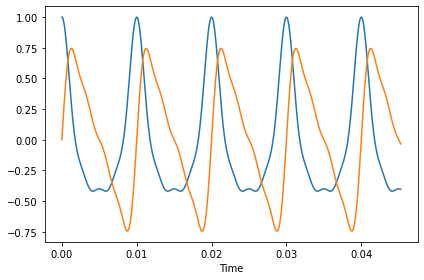
\includegraphics[width=0.75\textwidth]{task1.png}
		\caption{Вещественная и мнимая части комплексной синусоиды}
		\label{fig:task1}
	\end{figure}
	Действительная часть - смесь косинусов, а мнимая часть - смесь синусов. Они содержат одни и те же частотные компоненты с одинаковыми амплитудами, поэтому для нас они звучат одинаково.
	\begin{lstlisting}[language=Python,caption=Применим функцию с матричным умножением]
		def synthesize2(amps, freqs, ts):
			args = np.outer(ts, freqs)
			M = np.exp(1j * PI2 * args)
			ys = np.dot(M, amps)
			return ys
	
		amps = np.array([0.6, 0.25, 0.1, 0.05])
		ys = synthesize2(amps, freqs, ts)
		wave = Wave(ys.real, framerate)
		phi = 1.5
		amps2 = amps * np.exp(1j * phi)
		ys2 = synthesize2(amps2, freqs, ts)
		n = 500
		plt.plot(ts[:n], ys.real[:n], label=r'$\phi_0 = 0$')
		plt.plot(ts[:n], ys2.real[:n], label=r'$\phi_0 = 1.5$')
	\end{lstlisting}
	\begin{figure}[H]
		\centering
		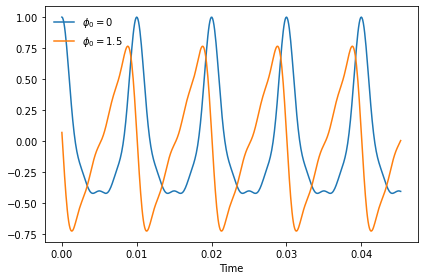
\includegraphics[width=0.75\textwidth]{task2.png}
		\caption{Повернули амплитуду на 1,5 радиана}
		\label{fig:task2}
	\end{figure}
	Поворот компонентов с одиновым смещением фазы изменил форму сигнала. Компоненты имеют разные периоды, и одно и то же смещение оказывает различное влияние на каждый компонент.

	\chapter{Анализ}
	Попробуем вычислить комплексные амплитуды компонент, зная частоты сигнала.
	\begin{lstlisting}[language=Python,caption=Применение первой функции для анализа]
		def analyze1(ys, freqs, ts):
			args = np.outer(ts, freqs)
			M = np.exp(1j * PI2 * args)
			amps = np.linalg.solve(M, ys)
			return amps

		n = len(freqs)
		amps2 = analyze1(ys[:n], freqs, ts[:n])
		N = 4
		ts = np.arange(N) / N
		freqs = np.arange(N)
		args = np.outer(ts, freqs)
		M = np.exp(1j * PI2 * args)
		MstarM = M.conj().transpose().dot(M)
	\end{lstlisting}
	Получилась унитарная матрица с точностью до дополнительного фактора \texttt{N}. Значит, ответ правильный.
	\begin{lstlisting}[language=Python,caption=Применение второй функции для анализа]
		def analyze2(ys, freqs, ts):
			args = np.outer(ts, freqs)
			M = np.exp(1j * PI2 * args)
			amps = M.conj().transpose().dot(ys) / N
			return amps

		N = 4
		amps = np.array([0.6, 0.25, 0.1, 0.05])
		freqs = np.arange(N)
		ts = np.arange(N) / N
		ys = synthesize2(amps, freqs, ts)
		amps3 = analyze2(ys, freqs, ts)
	\end{lstlisting}
	Снова получили правильный результат с точностью до ошибок округления.
	\begin{lstlisting}[language=Python,caption=Улучшение функции]
		def synthesis_matrix(N):
			ts = np.arange(N) / N
			freqs = np.arange(N)
			args = np.outer(ts, freqs)
			M = np.exp(1j * PI2 * args)
			return M

		def dft(ys):
			N = len(ys)
			M = synthesis_matrix(N)
			amps = M.conj().transpose().dot(ys)
			return amps
	\end{lstlisting}
	Полученный результат совпал с ответом функции \sloppy{\texttt{np.fft.fft}} в пределах ошибок округления.

	\chapter{Реальные сигналы}
	Протестируем полученную функцию \sloppy{\texttt{DFT}} на реальных сигналах.
	\begin{lstlisting}[language=Python,caption=Тест на реальном сигнале]
		from thinkdsp import SawtoothSignal

		framerate = 10000
		signal = SawtoothSignal(freq = 500)
		wave = signal.make_wave(duration=0.1, framerate=framerate)
		hs = dft(wave.ys)
		amps = np.abs(hs)
		plt.plot(amps)
	\end{lstlisting}
	\begin{figure}[H]
		\centering
		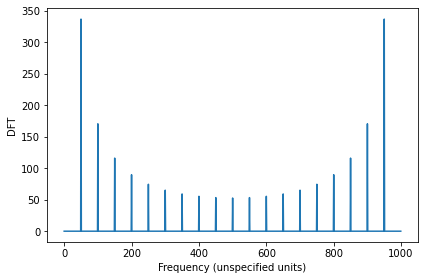
\includegraphics[width=0.75\textwidth]{task3.png}
		\caption{Результат}
		\label{fig:task3}
	\end{figure}
	\begin{lstlisting}[language=Python,caption=Берём левую половину сигнала]
		N = len(hs)
		fs = np.arange(N) * framerate / N
		plt.plot(fs[:(N // 2 + 1)], amps[:(N //2 + 1)])
	\end{lstlisting}
	\begin{figure}[H]
		\centering
		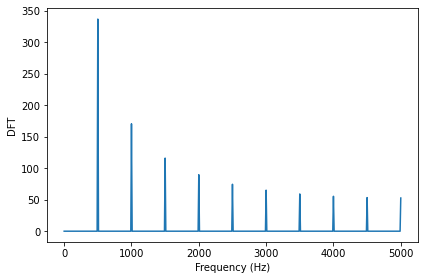
\includegraphics[width=0.75\textwidth]{task4.png}
		\caption{Первая половина сигнала}
		\label{fig:task4}
	\end{figure}
	\begin{lstlisting}[language=Python,caption=Сравнение реального сигнала с комплексным]
		from thinkdsp import TriangleSignal

		wave = TriangleSignal(freq = 1).make_wave(duration = 1, framerate = 8)
		wave2 = ComplexSinusoid(freq = 1).make_wave(duration = 1, framerate = 8)
		plt.plot(wave2.ts, wave2.ys.real)
		plt.plot(wave2.ts, wave2.ys.imag)

		hs = np.fft.fft(wave.ys)
		plt.plot(abs(hs))
		
		hs = np.fft.fft(wave2.ys)
		plt.plot(abs(hs))
	\end{lstlisting}
	\begin{figure}[H]
		\centering
		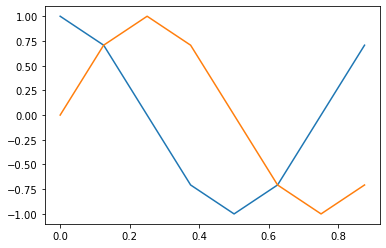
\includegraphics[width=0.75\textwidth]{task5.png}
		\caption{Комплексная синусоида}
		\label{fig:task5}
	\end{figure}
	\begin{figure}[H]
		\centering
		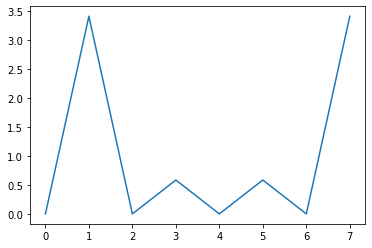
\includegraphics[width=0.75\textwidth]{task6.png}
		\caption{FFT реального сигнала - симметричный}
		\label{fig:task6}
	\end{figure}
	\begin{figure}[H]
		\centering
		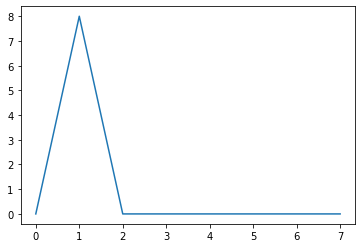
\includegraphics[width=0.75\textwidth]{task7.png}
		\caption{FFT комплексного сигнала - несимметричный}
		\label{fig:task7}
	\end{figure}
	
	\chapter{Упражнения}
	\section{Задание 2}
	Рекурсивный алгоритм для \sloppy{\texttt{DFT}} по лемме Дэниелсона-Ланцоша.

	\begin{align}
        		DFT(y)[n] = DFT(e)[n] + e^{-\frac{2\pi in}{N}}\cdot DFT(o)[n]
    	\end{align}
	где DFT(y)[n] - $n$-ый элемент DFT от $y$, \\
		e - массив сигнала, содержащий только четные элементы $y$ \\
		o - только нечетные элементы $y$.
	\begin{lstlisting}[language=Python,caption=Функция DFT]
		def dft(ys):
			N = len(ys)
			ts = np.arange(N) / N
			freqs = np.arange(N)
			args = np.outer(ts, freqs)
			M = np.exp(1j * PI2 * args)
			amps = M.conj().transpose().dot(ys)
			return amps
	\end{lstlisting}
	Сравнили результат её работы с ответом функции \sloppy{\texttt{np.fft.fft}}. Результаты совпали.
	\begin{lstlisting}[language=Python,caption=Функция для разделения исходного массива пополам]
		def fft_norec(ys):
			N = len(ys)
			He = np.fft.fft(ys[::2])
			Ho = np.fft.fft(ys[1::2])
			ns = np.arange(N)
			W = np.exp(-1j * PI2 * ns / N)
			return (np.tile(He, 2) + W * np.tile(Ho, 2))
	\end{lstlisting}
	Проверили её работу - всё правильно.
	\begin{lstlisting}[language=Python,caption=Итоговая функция]
		def fft(ys):
			N = len(ys)
			if N == 1: return ys    
			He = fft(ys[::2])
			Ho = fft(ys[1::2])
			ns = np.arange(N)
			W = np.exp(-1j * PI2 * ns / N)
			return (np.tile(He, 2) + W * np.tile(Ho, 2))
	\end{lstlisting}
	Также получили правильные результаты. Эта реализация алгоритма работает за $n \log n$ и занимает $n \log n$ памяти. Возможно, его можно улучшить.

	\chapter{Вывод}
	В данной работе мы изучили дискретное преобразование Фурье и раелизовали алгоритмы для его использования с различными сигналами. В последнем упражнении нам удалось немного улучшить полученный алгоритм.
\end{document}